% !TeX spellcheck = en_US

\chapter{Design overview}


\begin{figure}
	\centering
	\begin{subfigure}[b]{0.45\textwidth}
		\centering
		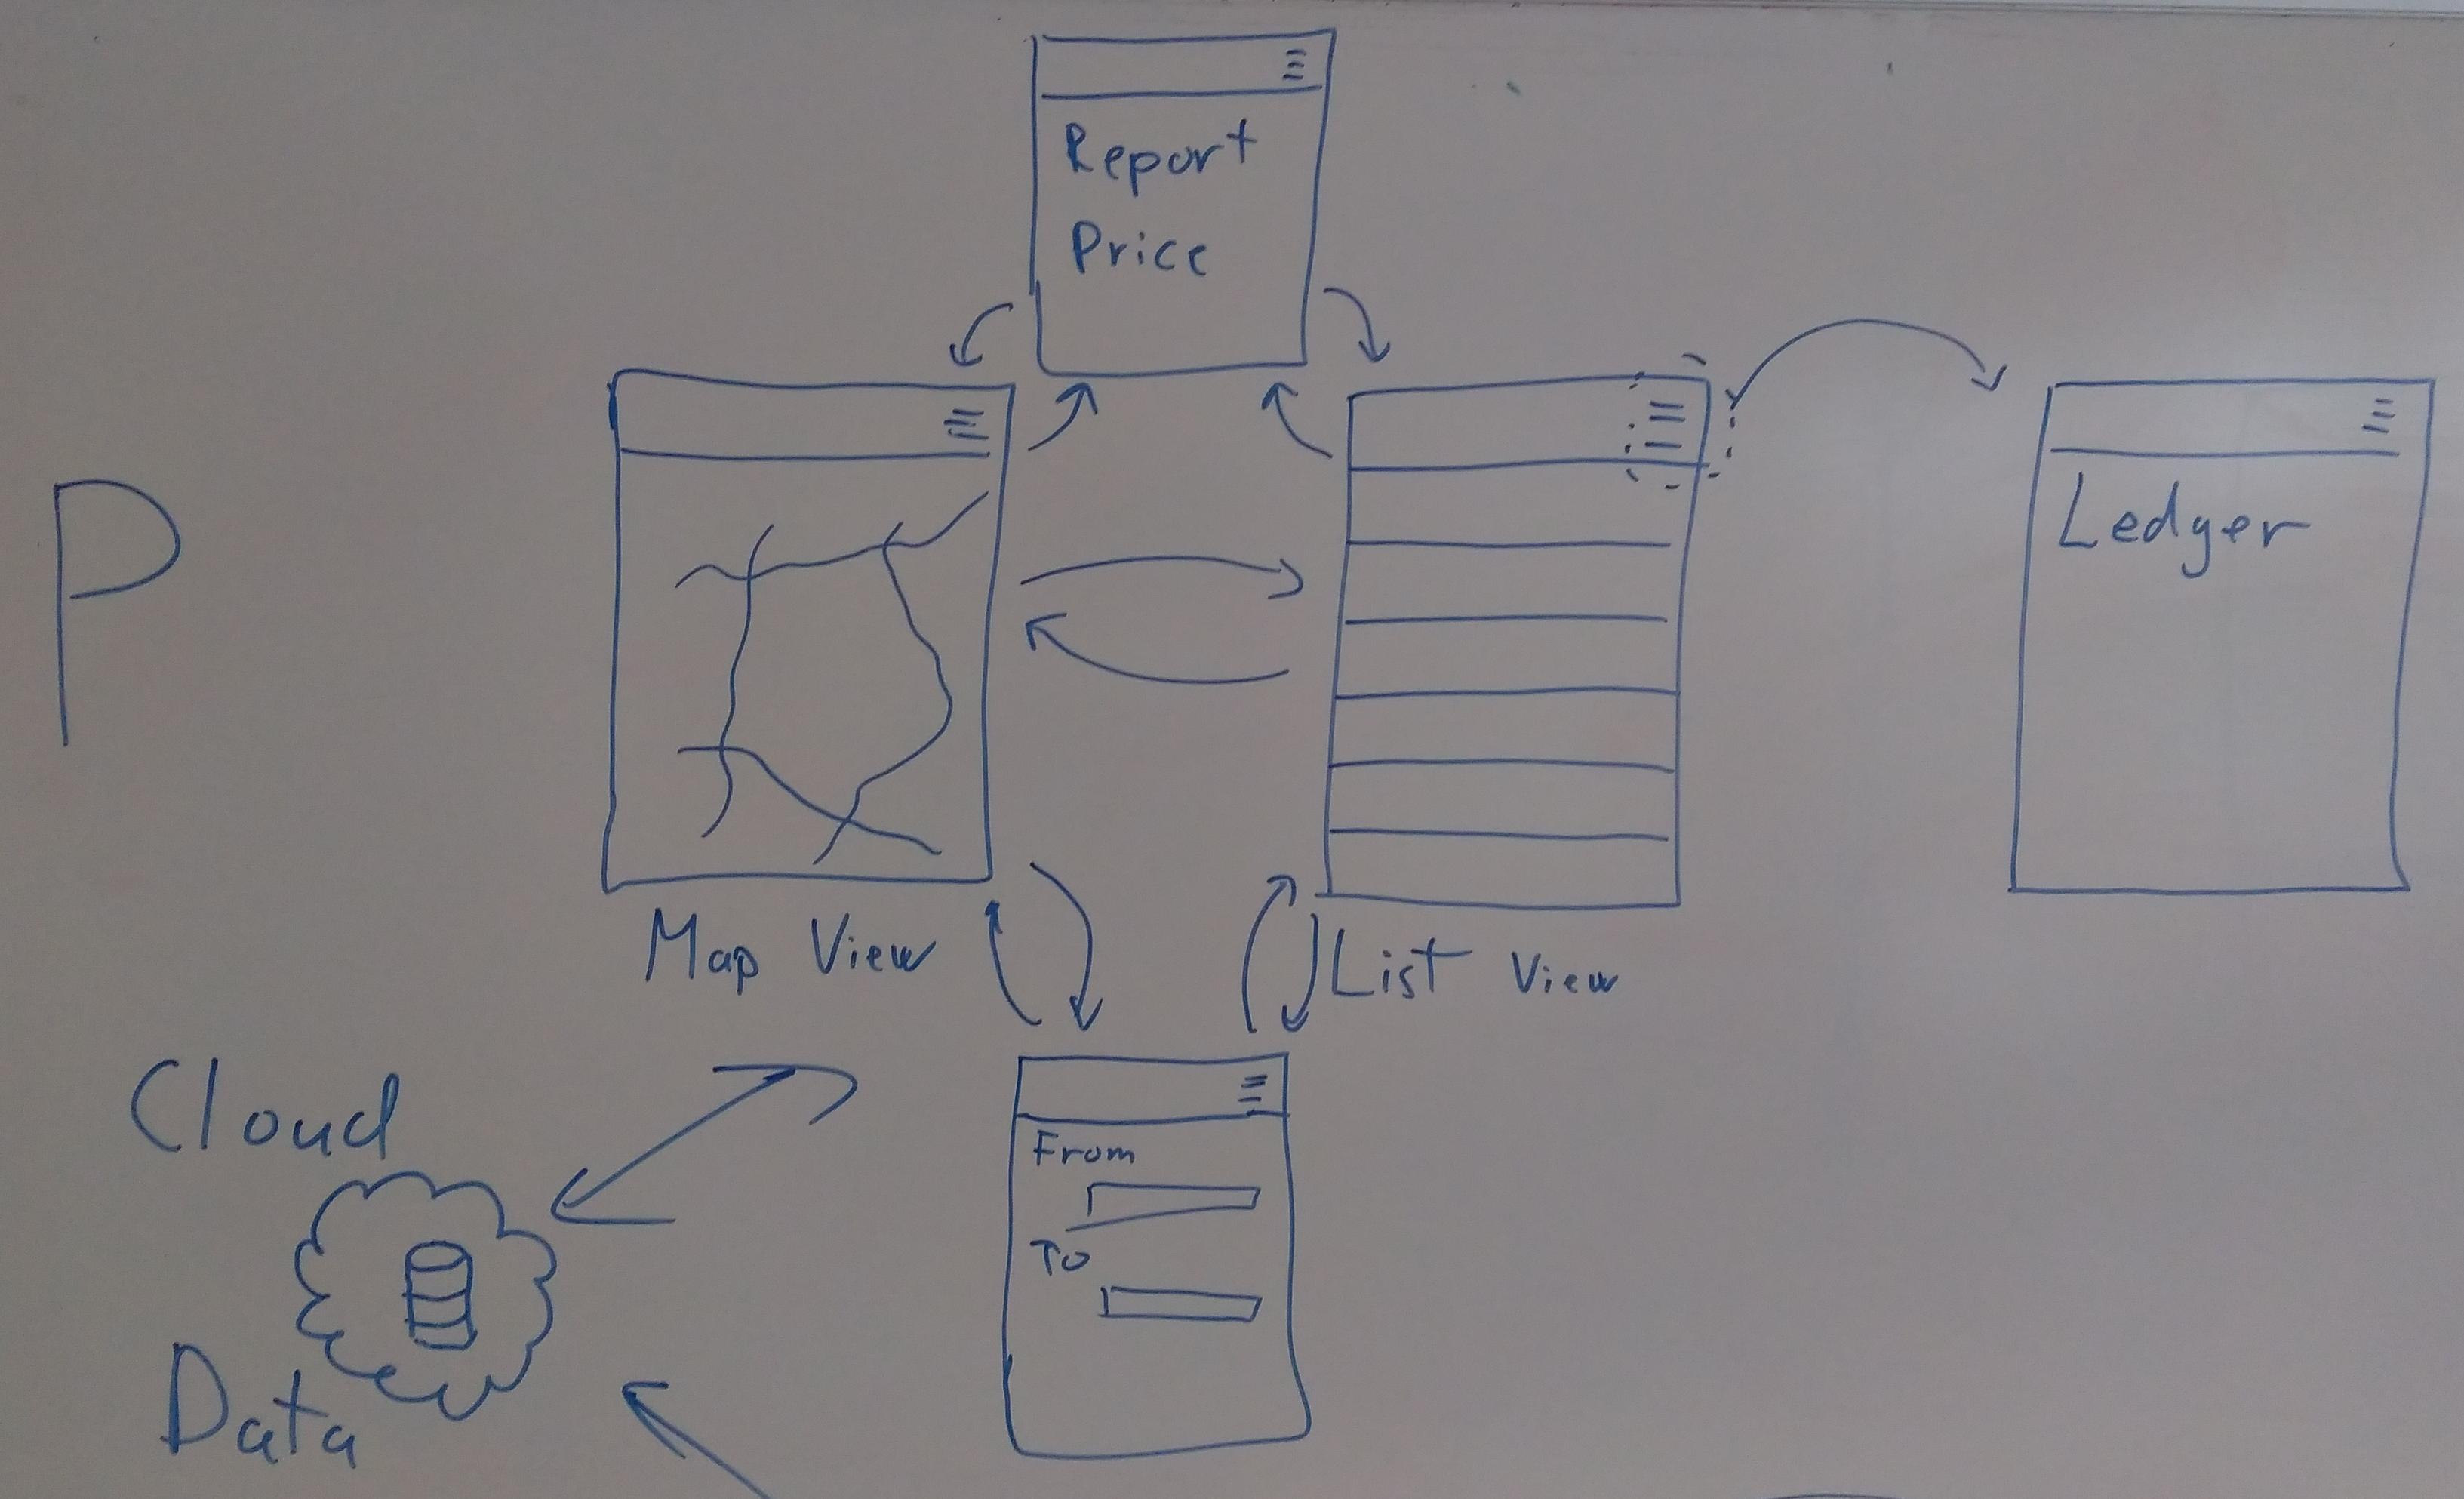
\includegraphics[width=\textwidth]{P.jpg}
		\caption{Overview for the main portrait flow.}
		\label{fig:p}
	\end{subfigure}
	\quad
	\begin{subfigure}[b]{0.45\textwidth}
		\centering
		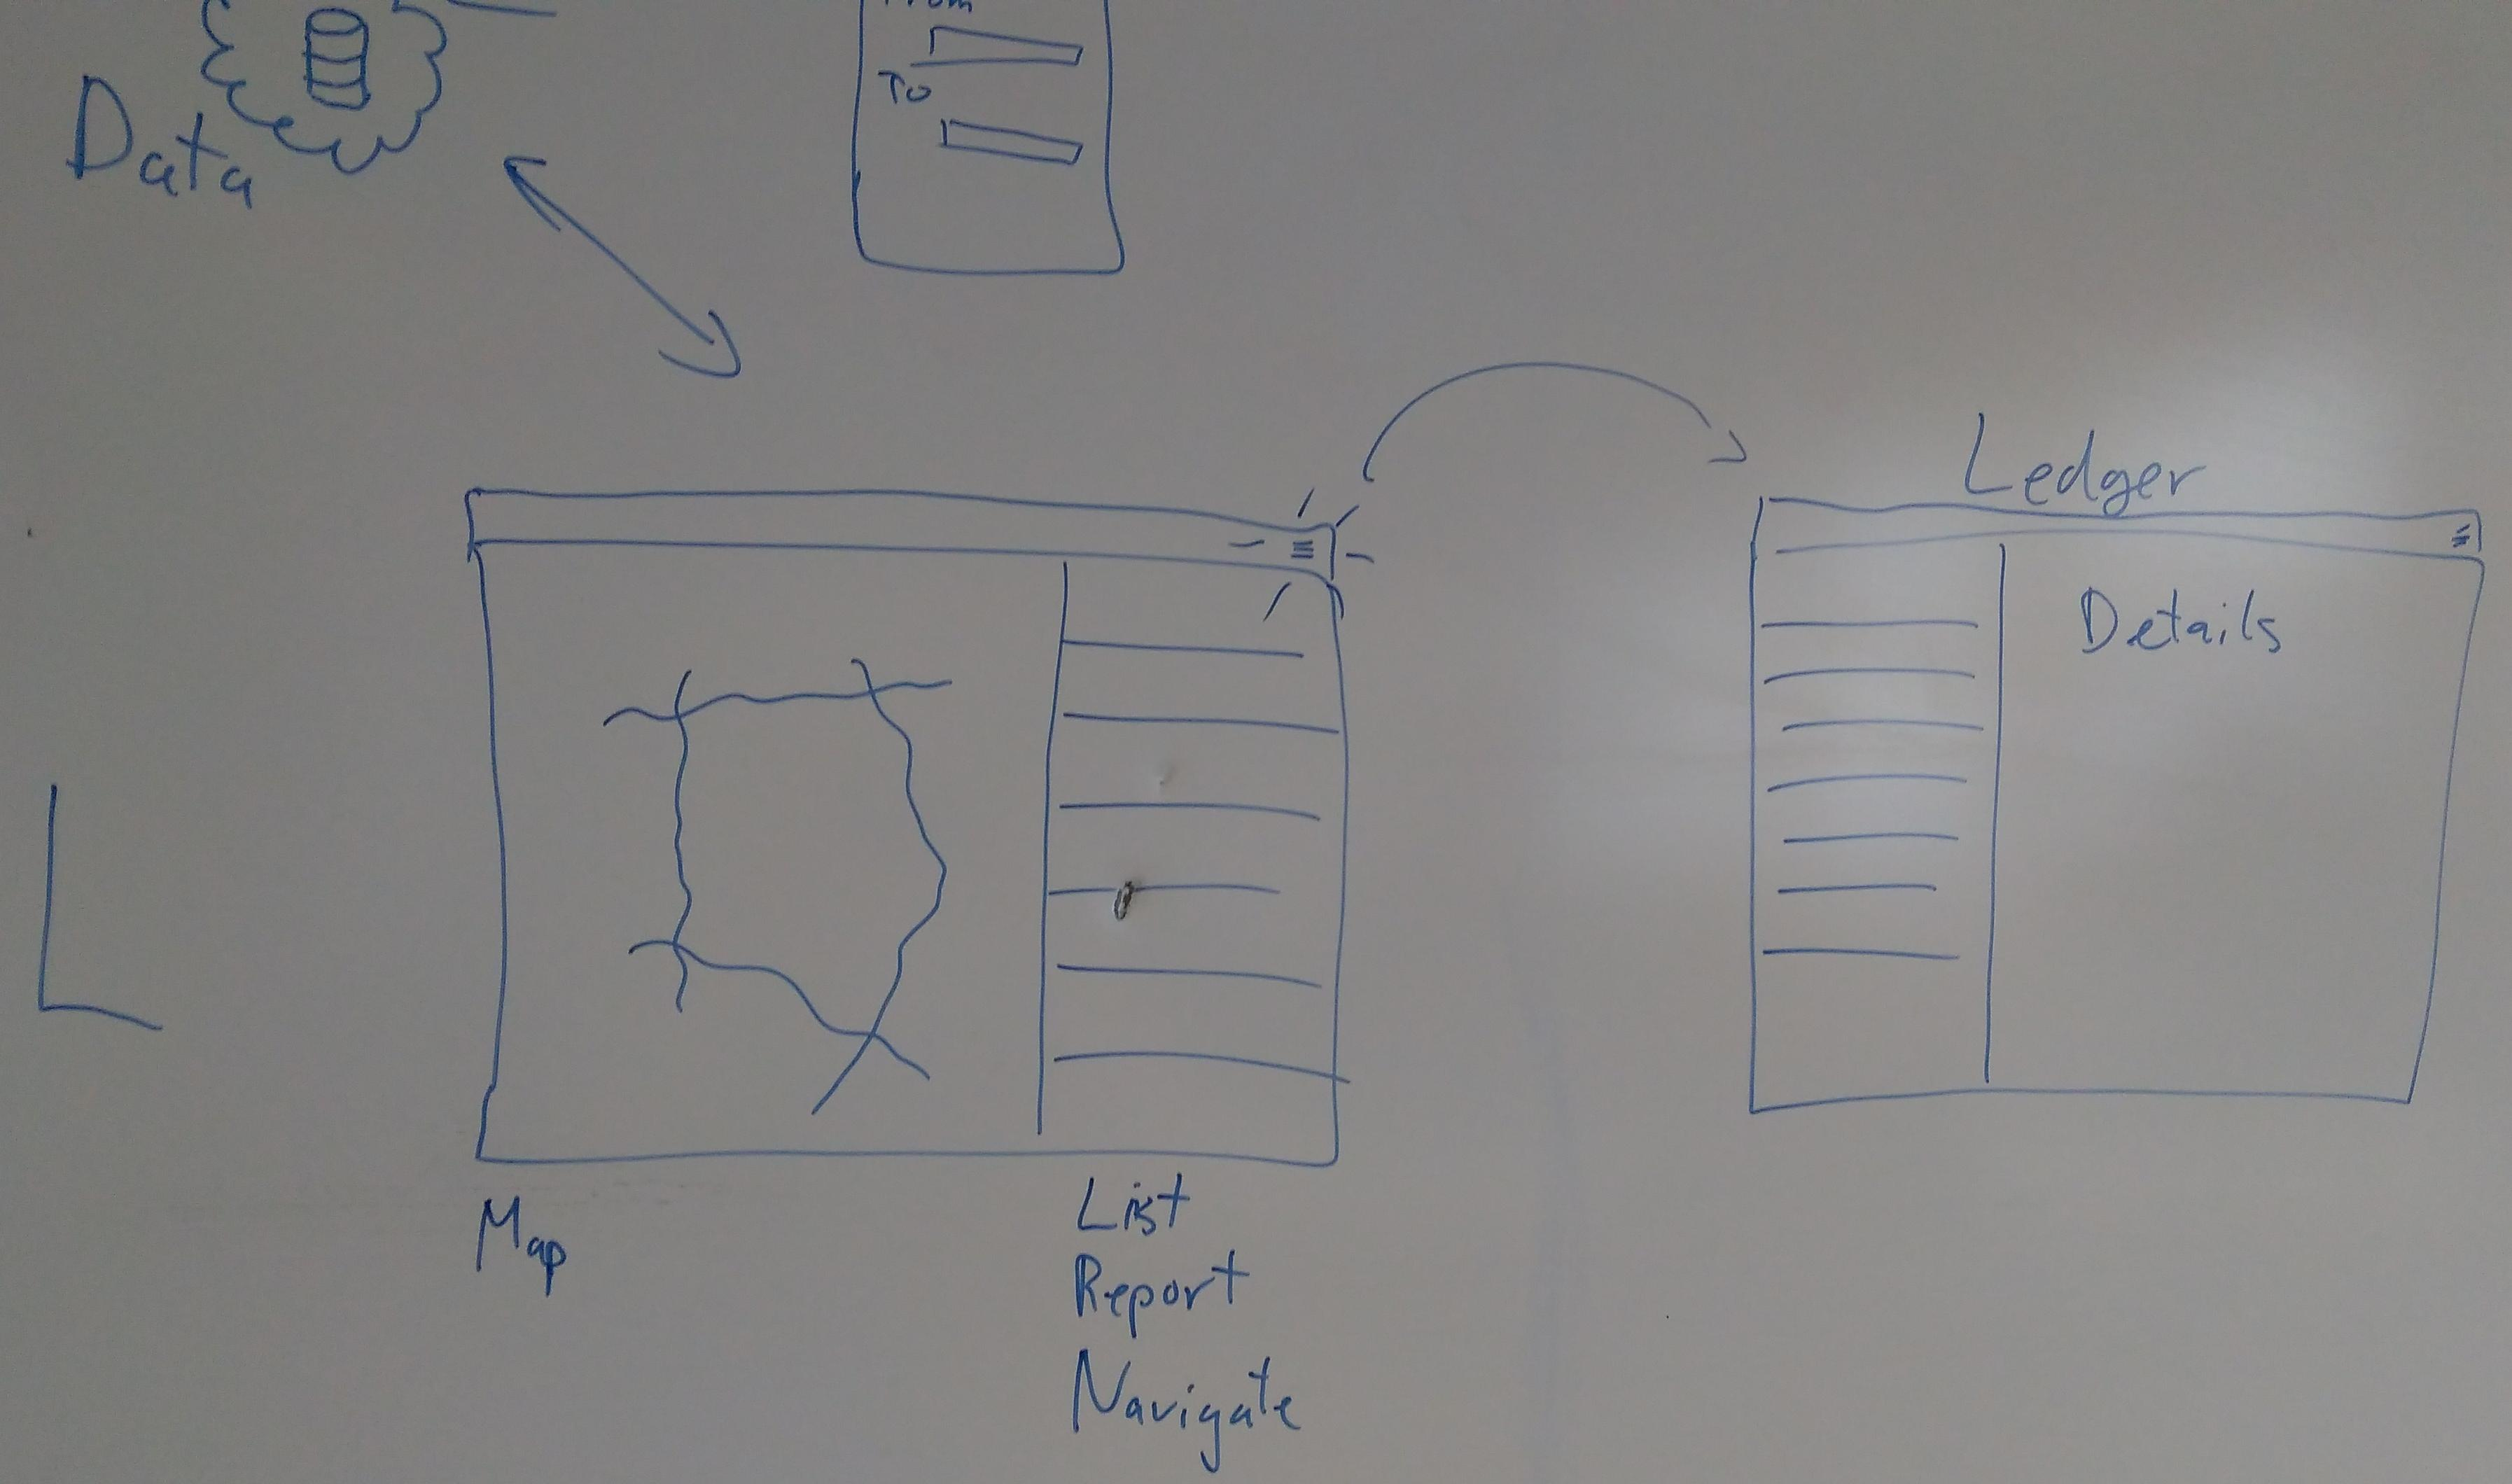
\includegraphics[width=\textwidth]{L.jpg}
		\caption{Overview for the main tablet/landscape flow.}
		\label{fig:l}
	\end{subfigure}
	\caption{Views of the flow in portrait and landscape orientation.}
\end{figure}


\section{Activities}
The application will be designed for usage in portrait mode on hand-held devices, as well as landscape mode on larger devices e.g. tablets. Since the layout changes, the design of the application also changes to a large degree, in order to deliver the best possible user flow in each case.

\subsection{Portrait}
I portrait mode it will include the following activities:
\begin{itemize}
	\item Setup/options screen
	\item Map mode (Default)
	\item List mode
	\item Show prices
	\item Route mode
	\item Report prices
	\item View ledger
	\item Enter ledger information
\end{itemize}

\subsection{Landscape}
In landscape mode, the dynamics of user operation has changed, and fragments will instead be used to alter the content of our activities, depending on the user action. In landscape mode, the different activities is expected to be:
\begin{itemize}
	\item Setup/options screen
	\item Main screen
	\item View ledger
\end{itemize}

The main screen is split into two pieces, each showing a different fragment. For instance, it could be the map mode from portrait on the left side, and the right side would show the prices of the last selected station. The map mode could be swapped for the list view while still keeping the prices list. While at a station, the 'show prices' fragment could be replaced by a 'report prices' fragment. When planning a route, the map fragment would be shown in union with the 'route mode' fragment.

\section{Risks}
A high degree of fragmentation between the portrait and landscape modes.
The requirement for backend API.
The acquisition of data.